
%(BEGIN_QUESTION)
% Copyright 2007, Tony R. Kuphaldt, released under the Creative Commons Attribution License (v 1.0)
% This means you may do almost anything with this work of mine, so long as you give me proper credit

Brytere, om de er operert for hånd, en aktuator eller en fysiks prosess, kommer i to varianter: \textit{normwlt åpen} og \textit{normalt lukket}. Du er sikkert vant til å se begge typer i skjemaer. 

$$\includegraphics[width=15.5cm]{i02966x01.eps}$$

\textit{Normalt åpne brytere} lukker (slepper strøm i gjennom) når de aktiveres. Når de deaktiveres, går tilbake til utgangposisjonen eller normalposisjonen. 

\textit{Normalt-lukkede brytere} er helt motsatt: de åpner (stopper strømmen) når de aktiveres og går tilbake til lukket (normal) posisjon nå de deaktiveres. 

\vskip 10pt

Definer "normalposisjonen" for disse bryterene. Med andre ord forklar hvilken prosess egenskap som må til for å holde den i normalposisjon og hva som  aktiverer den. 

$$\includegraphics[width=15.5cm]{i02966x02.eps}$$


\underbar{file i02966}
%(END_QUESTION)





%(BEGIN_ANSWER)

The ``normal'' condition for a process switch is the condition of {\it least stimulus}.  For example:

\vskip 10pt

\begin{itemize}
\item{} A pressure switch will be in its ``normal'' state when there is {\it minimum pressure applied}
\vskip 10pt
\item{} A level switch will be in its ``normal'' state when there is {\it no level detected by the switch}
\vskip 10pt
\item{} A temperature switch will be in its ``normal'' state when it is {\it cold}
\vskip 10pt
\item{} A flow switch will be in its ``normal'' state when there is {\it no flow detected by the switch}
\end{itemize}

%(END_ANSWER)





%(BEGIN_NOTES)

The ``normal'' status of an electrical switch, as universally defined by manufacturers, is a condition of:

\begin{itemize}
\item{} minimum stimulus
\item{} rest
\item{} a ``low'' sensing condition
\end{itemize}

Normally-Open (NO) contacts are sometimes called {\it form-A} contacts.

\vskip 10pt

Normally-Closed (NC) contacts are sometimes called {\it form-B} contacts.

\vskip 10pt

A switch having both NO and NC contacts is sometimes called {\it form-C}.



%INDEX% Switch, ``normal'' status

%(END_NOTES)


